\chapter{PIVlab PROGRAMSKI PAKET}
\label{chap:Poglavlje5}

U današnje vrijeme primjena PIV mjerenja postala je sve češća, te je PIV gotovo implementiran u svako područje dinamike fluida gdje brzine i pomaci trebaju biti kvantificirani, od istraživanja do razvoja. U te svrhe na tržištu su se pojavili brojni komercijalni PIV softveri (npr. Dantec DynamicStudio, ILA PIVview, LaVision Flowmaster, TSI INSIGHT), koji često nisu limitirani samo na 2D PIV mjerenja, nego u svoje sučelje imaju uključena i 3D (stereo) mjerenja, te još napredniju obrade podataka (volumetrijski PIV). Također postoje i brojni open-source PIV softveri ( JPIV\cite{jpiv}, Fluidimage\cite{fluidimage}, Fluere\cite{fluere}, mpiv\cite{mpiv}, UVMAT\cite{uvmat}, OpenPIV\cite{openpiv}) koji se isto tako mogu koristiti u znanstvene svrhe.
\par
U ovom radu koristi se open-source PIVlab\cite{thielicke2021PIVinMatLab} softver koji je prvotno objavljen 2010 godine, te se aktivno održava i ažurira i danas.  PIVlab je implementiran kao besplatni toolbox i aplikacija u programski jezik MATLAB. Na \textit{Slici \ref{sl:5.1}} prikazan je dijagram toka rada i opcija koje nudi PIVlab sučelje. Sa slike je vidljivo kako PIV analiza započinje sa učitavanjem snimki (ulaz), te završava sa "izbacivanje" izlaznih podataka. U ovom poglavlju ukratko će biti objašnjene i prikazane većina opcija i koje PIVlab nudi. Obično se cjelokupna analiza izvršava u PIVlab grafičkom sučelju (PIVlab\_GUI.m), no moguća je kontrola i bez sučelja koristeći command-line.
\begin{figure}[h]  
	\centering
	%\usepackage{graphicx}
	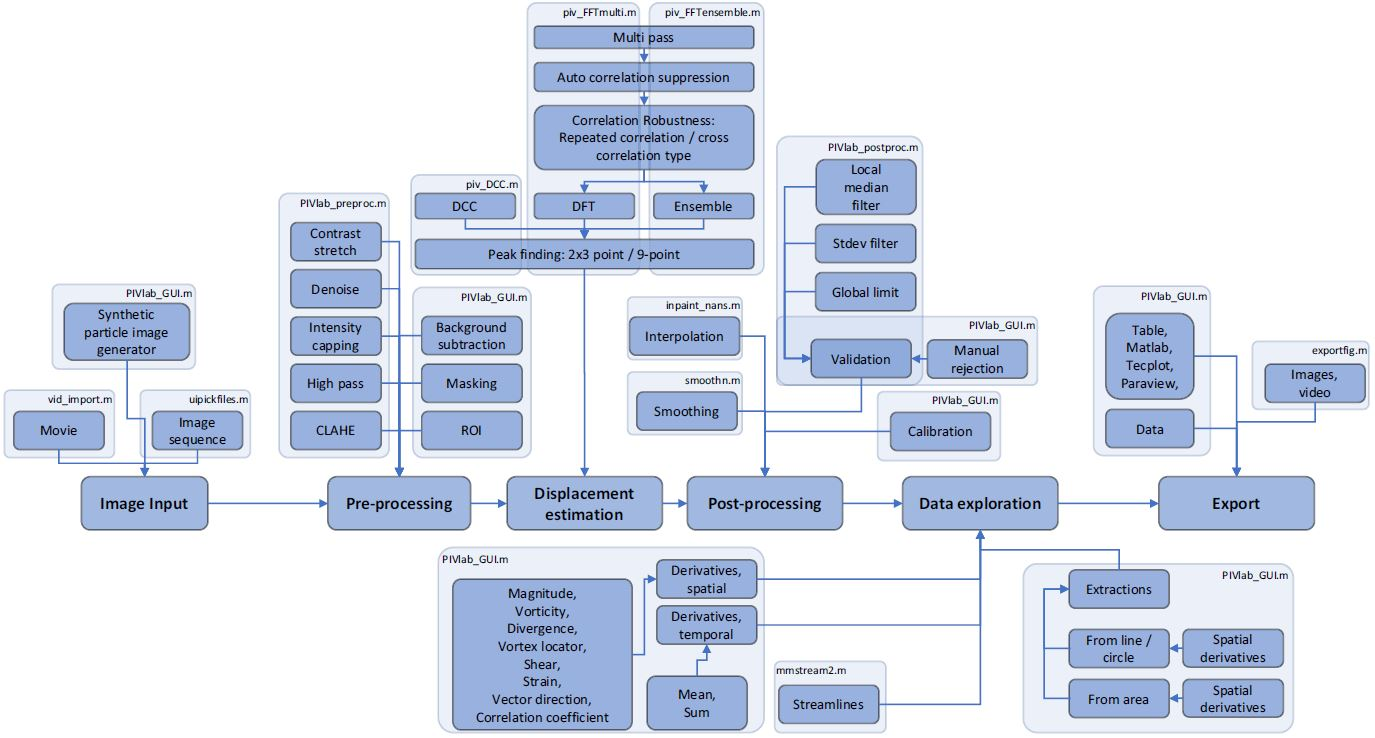
\includegraphics[width=16.6cm]{./5_PIVlab/slika5_1.jpg} 
	\caption{Arhitektura i dijagram toka PIVlab-a \cite{thielicke2021PIVinMatLab}}
	\label{sl:5.1}
\end{figure}
\par
U najnoviju verziju PIVlab softvera implementirana su brojna poboljšanja. U nastavku će samo neka bitnija poboljšanja biti ukratko objašnjena radi lakšeg razumijevanja načina rada softvera.
\begin{description}[style=unboxed,leftmargin=0cm]
	\item[Korelacija skupine snimki (\textit{eng. ensemble correlation})] Pristup korelacija skupine snimki PIV mjerenjima temelji se na usrednjavanju korelacijskih matrica svih dostupnih snimki prije nego što nastupi pronalazak korelacijskog vrha, te sama procjena srednjeg pomaka čestica. Generalno ova tehnika procesiranja koristi se najviše u PIV mjerenjima gdje je gustoća distribucija čestica markera mala (npr. $\mu$PIV). Usrednjavanjem matrica dobije se konačna korelacijska matrica (\textit{Slika \ref{sl:5.2}}) u kojoj je omjer signal-šum mnogo bolji odnosno veći. Veliki nedostatak ovog pristupa je taj što strujanje mora biti stacionarno, tj. ne smije se mijenjati u vremenu, što je i logično jer tada bi imali različite brzine u različitim trenucima snimki, što bi rezultiralo u proširenom korelacijskom vrhu čija detekcija bi bila neuspješna.
	\begin{figure}[H]  
		\centering
		%\usepackage{graphicx}
		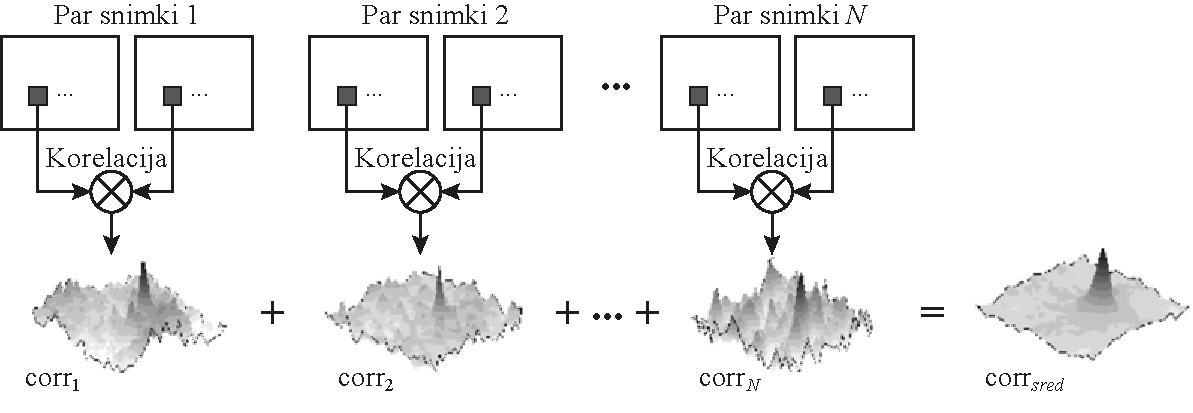
\includegraphics[width=16cm]{./5_PIVlab/slika5_2.pdf} 
		\caption{Koncept pristupa adaptivnoj korelaciji skupine snimki \cite{willert2008ensemble}}
		\label{sl:5.2}
	\end{figure}
	Na \textit{Slici \ref{sl:5.2}} jasno je uočljiva velika prednost ove tehnike, naime na posljednjoj usrednjenoj korelacijskoj ravnini vidljiv je značajan gubitak šuma nego na svakoj korelaciji posebno.
	\item[Poboljšanje korelacijskoj algoritma - kružna i linearna korelacija] PIVlab ima mogućnost primjene direktne kros-korelacije (DKK) u prostornoj domeni, te kros-korelacije signala u frekvencijskoj domeni koristeći diskretnu Fourierovu transformaciju (DFT). DFT algoritam je 30 do 50\% brži od DKK ovisno o implementaciji. PIVlab tipično koristi kružnu kros-korelaciju kako bi izveo DFT, kružna kros-korelacija pretpostavlja kako je signal periodičan, što naravno nije realan slučaj, te radi toga ova pretpostavka unosi frekvencije u DFT spektar koje inače ne postoje\cite{raffel2018_book}. Kako bi se izbjegao ovaj negativan učinak, signal može biti nuliran na granicama, što dovodi do linearne, ne-periodične kros-korelacije. Kako tipični podaci u snimkama imaju određeni šum (pozadinski signal koji različit od nule), nuliranje dovodi od rubnog diskontinuiteta, koji ponovno uništava spektar DFT analize i kros-korelacijski signal. Efekt "oštrih rubova" može biti oslabljen oduzimanjem prosječne vrijednosti intenziteta iz ulaznih snimki.
	\item[Poboljšanje korelacijskog algoritma - ponovljena korelacija] Još jedna tehnika da se dobije robusnija kros-korelacija je "ponavljanje korelacije". Ova metoda služi kao "ne-naknadno ispitivanje" kako bi se smanjio broj nepravilno dobivenih vektora brzine. Naime ova tehnika poboljšava dobivanje podataka kod snimki sa lošim omjerom signal-šuma, kros-korelacija se ne izvršava samo jednom za svaku procjenu pomaka, nego ukupno pet puta. Prozori ispitivanja se pomiču, gore-lijevo, gore-desno, dolje-lijevo i dolje-desno za 25\% duljine prozora ispitivanja. Dobivene korelacijske matrice se potom množe, što rezultira u novoj matrici koja ima manje šuma, te više izraženim vrhovima. Svaka korelacijska vrijednost koja nije prisutna u samo jednoj od pet korelacijskih matrica tako je izbačena iz konačne korelacijske matrice. Osnovne opcije koje sadrži PIVlab softver prikazane su u \textit{Tablici \ref{tab:5.1}}, naravno ove opcije se mogu i dodatno naštimati, ali za prosječnu analizu dovoljne su zadane tri postavke.
	\begin{table}[h]
		\centering
		\caption{Osnovne postavke korelacijskog algoritma u PIVlabu \cite{thielicke2021PIVinMatLab}}
		\begin{tabular}{|l|llll|}
			\hline
			\rowcolor[HTML]{C0C0C0} 
			{\color[HTML]{000000} \textbf{\begin{tabular}[c]{@{}l@{}}Robusnost \\ korelacije\end{tabular}}} & {\color[HTML]{000000} \textbf{\begin{tabular}[c]{@{}l@{}}Tehnika \\ deformacije \\ prozora\end{tabular}}} & {\color[HTML]{000000} \textbf{\begin{tabular}[c]{@{}l@{}}Kros-\\ korelacija\end{tabular}}} & {\color[HTML]{000000} \textbf{\begin{tabular}[c]{@{}l@{}}Ponovljena \\ korelacija\end{tabular}}} & {\color[HTML]{000000} \textbf{\begin{tabular}[c]{@{}l@{}}Vrijeme \\ izvršenja\end{tabular}}} \\ \hline
			\textbf{"Standard"}                                                                              & linearna                                                                                                  & kružna                                                                                     & isključeno                                                                                       & +                                                                                            \\
			\textbf{"High"}                                                                                  & spline                                                                                                    & linearna                                                                                   & isključeno                                                                                       & ++                                                                                           \\
			\textbf{"Extreme"}                                                                               & spline                                                                                                    & linearna                                                                                   & uključeno                                                                                        & ++++                                                                                         \\ \hline
		\end{tabular}
	\label{tab:5.1}
	\end{table}
	\item[Eliminacija pozadine] Neravnomjerno osvjetljenje, te ostali mogući pozadinski efekti u snimkama mogu rezultirati dodatnom procjenom nepravilnih vektora. Ovaj neželjeni efekt gdje pozadina daje visok postotak šuma u korelacijskoj ravnini može biti eliminiran na način da se izračuna prosječna vrijednost svih dostupnih snimki te da se dobivena vrijednost oduzme od svake snimke posebno.
	\item[Potiskivanje auto-korelacije] Još jedna od metoda poboljšanja PIV mjerenja je potiskivanje stacionarnog pozadinskog signala u korelaciji. Kao što je već ranije objašnjeno auto-korelacija je množenje snimke same sa sobom, što rezultira nepostojanjem pomaka. U ovom slučaju do auto-korelacije dolazi (iako su korelirane dvije različite snimke) zbog toga što pozadinski signal (šum) dominira nad korelacijom, a dostupan je samo jedan par snimki, te tada korištenje eliminacije pozadine nije moguće. U tom slučaju se korelacija uhvati za pozadinski signal (šum) što rezultira nultim pomakom (auto-korelacija). Ovo je moguće izbjeći na način da se maskira centralni vrh u korelacijskoj matrici. Tada će pronalaženje vrha detektirati drugi najveći vrh korelacijske ravnine, koji je najvjerojatnije stvarni pomak. Naravno korištenje ove tehnike treba limitirati na slučajeve u kojima zasigurno pomak nikad nije nula.
\end{description}